\documentclass[xcolor=table]{beamer}

\usepackage[utf8]{inputenc}
\usepackage[french]{babel}

% TODO 1. Remplir les champs
\newcommand{\mytitle}{Cthulhu Dark, version française}
\newcommand{\myauthor}{Olivier Rey}
\newcommand{\mysubject}{Jeu de rôles}
\newcommand{\mykeywords}{JDR,TTRPG,RPG,orey,cthulhu,lovecraft,horreur}
\newcommand{\myversion}{3.0}
\newcommand{\mycolor}{violet}     % green pour le fond noir
\newcommand{\mylinkcolor}{blue}   % red pour le fond noir
\newcommand{\myrepo}{jdr-risus}
\newcommand{\myheader}{{\Huge R}{\huge ISUS}}
\newcommand{\myreference}{OReyJdr13}

%\usepackage[orientation=portrait,size=a4,scale=1.4,debug]{beamerposter}
\usepackage[orientation=portrait,size=a4, scale=1.48]{beamerposter}

% TODO 2. Couleur des tables
\definecolor{lightgray}{gray}{0.85}     % white version; black version 0.15
\definecolor{verylightgray}{gray}{0.95} % white version; black version 0.05
\let\oldtabular\tabular
\let\endoldtabular\endtabular
\renewenvironment{tabular}{\small\rowcolors{1}{lightgray}{verylightgray}\oldtabular}{\endoldtabular}

%%\usepackage{graphicx}
\graphicspath{{../yed/}{../images/}}

% to use \textcopyleft
\usepackage{textcomp}

\usepackage{comment}

\usepackage{wrapfig}

\usepackage{amssymb}

\begin{comment}

\mode<presentation>
{
\usetheme{Berlin}
%\usetheme{Dreuw}
}
\end{comment}

% caractéristiques
\title[Risus]{Écran Risus avec les règles complètes}
\author{Olivier Rey}
\institute{The Risus Intergalactic Consortium}
\date{May 14 2022}

% paramètres beamer
% Pas de barres de navigation
\beamertemplatenavigationsymbolsempty

% Marges sur le document
\setbeamersize{text margin left=1.5cm,text margin right=1.5cm}
\setbeamertemplate{headline}{\vspace{0.0cm}}
\setbeamertemplate{footline}{\vspace{1cm}}

% PDF features
\usepackage{hyperref}
\hypersetup{
  pdftitle={\mytitle},
  pdfauthor={\myauthor},
  colorlinks=true,
  linkcolor=\mylinkcolor, % white version
  urlcolor=\mylinkcolor, % white version
  pdfsubject={\mysubject},
  pdfkeywords ={\mykeywords},
  pdfstartview={FitH},
  bookmarksopen={false},
  bookmarksnumbered={true}
}

% POur utiliser \justifying dans les columns
\usepackage{ragged2e}

% Pour les images en mode maxi
%\usepackage{background}
%\backgroundsetup{contents={}}
\usepackage{pdfpages}

%============= Mes macros

% pour mon itemize
\usepackage{enumitem}
\usepackage{pifont}
\newlist{myitemize}{enumerate}{2}
%\setlist[myitemize,1]{label=-- \arabic*:}
%\setlist[myitemize,2]{label=\ding{217} \alph*)}
%\setlist[myitemize,1]{label=--}
\setlist[myitemize,1]{label=\ding{217}}
\setlist[myitemize,2]{label=\ding{217}}

\newcommand{\mybullet}{\ding{217}}

\newcommand{\mysection}[1]{
\vspace{0.2cm}
\noindent{\color{\mycolor}\large\textbf{#1}}
\vspace{0.1cm}
{\color{\mycolor}\hrule}
\vspace{0.2cm}
}

\newcommand{\mysubsection}[1]{
\vspace{0.1cm}
\noindent{\color{\mycolor}\emph{#1}}
}

\newcommand{\deuxcolonnes}[2]{
\begin{columns}[t]\begin{column}{.5\linewidth}
\justifying
#1\end{column}\begin{column}{.5\linewidth}
\justifying
#2\end{column}\end{columns}
}

%info alignements

\begin{comment}
\begin{tabular}%
  {>{\raggedright\arraybackslash}p{3.5cm}%
   >{\centering\arraybackslash}p{3.5cm}%
   >{\raggedleft\arraybackslash}p{3.5cm}%
  }
  \lipsum[1] & \lipsum[2] & \lipsum[3]
\end{tabular}
\end{comment}


%============================================
\begin{document}


%=======================================
\begin{frame}[t]

\deuxcolonnes{%col1
\begin{center}

\includegraphics[scale=0.60]{logo-risus-fr.png}
\end{center}

%======= mysection
% TODO Création du personnage
\mysection{Création du personnage}

%--- mysubsection
\mysubsection{Les clichés}

Risus n'utilise que des dés à 6 faces. Chaque PJ a un crédit de 10D de Création (noté 10D$\Subset$) à répartir sur des Clichés (entre 3 et 10, idéalement 4) librement choisis. Classiquement, un PJ est décrit par 4 Clichés à 4D, 3D, 2D et 1D.

\vspace{0.2cm}

\begin{tabular}{lc|lcc}
\textbf{Niveau du PJ} & \textbf{Nb de dés} & \textbf{Cliché}    & \textbf{Coût Cliché} & \textbf{Gonflette ?} \\
Débutant &  1D & Normal     & 1D$\Subset$ $\rightarrow$ 1D & Simple $^{1}$ \\
Professionnel & 3D & Magique    & 2D$\Subset$ $\rightarrow$ 1D & Double $^{2}$ \\
Expert, maître & 6D & Psioniques & 2D$\Subset$ $\rightarrow$ 1D & Double $^{2}$ \\
\end{tabular}

\vspace{0.2cm}

La table ci-dessus donne une idée du niveau du personnage en fonction de son nombre de dés dans un Cliché.

Attention, tous les clichés n'ont pas tous le même coût.

%--- mysubsection
\mysubsection{Gonflette et Double Gonflette}

\vspace{0.2cm}

\begin{tabular}{p{4.15cm}p{4.15cm}}
\textbf{$^{1}$ Gonflette}    & \textbf{$^{2}$ Double Gonflette}  \\
Accord du MJ & Accord du MJ \\
Le joueur choisit le nombre de dés de Gonflette : n & Le joueur choisit le nombre de dés de Gonflette : n \\
+nD pour un round de combat & +2nD pour un round de combat \\
-nD sur le cliché à partir du round suivant &-nD sur le cliché à partir du round suivant \\
Niveau Cliché entre parenthèses (ex. : Lutteur (3)) & Niveau Cliché entre crochets (ex. : Sorcier [3]) \\
\end{tabular}

\vspace{0.2cm}

%--- mysubsection
\mysubsection{Matériel ("Tools of the Trade")}

Inclus tant que cela reste logique et raisonnable pour le Cliché.

%--- mysubsection
\mysubsection{Options de création}

\vspace{0.2cm}

\begin{tabular}{p{2cm}p{6.3cm}}
\textbf{Option}    & \textbf{Description}  \\
Coups de Bol & 1D$\Subset$ = 3 Coups de Bol ; 1 Coup de Bol donne +1D sur une action. \\
Point Faible & Un point faible du PJ validé par le MJ = +1D$\Subset$. \\
Background   & S'il est bien fait, le MJ peut donner +1D$\Subset$. \\
\end{tabular}

\vspace{0.2cm}

%======= mysection
\mysection{Les 3 mécaniques du jeu}

\begin{myitemize}
\item L'action simple : jet contre un Facteur de Difficulté (FD) ("Target Number" ou "TN" en anglais)
\item Combat : basé sur le système du duel
\item Conflits à action unique (CAU)
\end{myitemize}


%======= mysection
% TODO Action simple
\mysection{1. Action simple : jet contre un FD}
L'action est réussie si le score est supérieur ou égal au FD.

\begin{wraptable}{l}{0pt}
\begin{tabular}{cl}
\textbf{FD} & \textbf{Difficulté de l'action} \\
\textbf{5} & Facile                          \\
\textbf{10} & Défi même pour un pro           \\
\textbf{15} & Défi héroïque                   \\
\textbf{20} & Difficulté presque surhumaine   \\
\textbf{30} & Difficulté surhumaine           \\
\end{tabular}
\end{wraptable}

Important : le FD est adapté au Cliché.

Par exemple, crocheter une serrure a un FD=7 pour un Voleur (3), FD=7+5=12 pour un Agent Secret (3) et FD=7+10=17 pour un Violoniste (3) (+0/+5/+10).

%======= mysection
% TODO Combat
\mysection{2. Combat : basé sur le système du duel}

\mysubsection{Types de combats}

Généralement, l'agresseur détermine le type de combat.

\vspace{0.2cm}

\begin{tabular}{>{\centering\arraybackslash}p{2.6cm}>{\centering\arraybackslash}p{2.6cm}>{\centering\arraybackslash}p{2.6cm}}
\textbf{Type de combat} & \textbf{Type de combat} & \textbf{Type de combat}\\
Débat & Courses de chevaux & Duel aérien \\
Duel astral & Duel psychique & Duel de banjos \\
Séduction & Tribunal & Combat physique \\
Duel de danse & Jeopardy & Etc. \\
\end{tabular}

\vspace{0.2cm}

Du type de combat dépend le type de Cliché utilisé.

Note : dans un combat, il est possible d'utiliser plusieurs Clichés différents, mais le premier Cliché à 0D fait perdre le combat.

}{%col2

\mysubsection{Round de combat}

\vspace{0.2cm}

\begin{tabular}{p{3cm}p{5.1cm}}
\textbf{Processus} & \textbf{Conséquence} \\
\textbf{1. Choisir le Cliché} & Le MJ détermine si le cliché est adapté ou pas $^{3}$ $^{4}$ \\
\textbf{2. Options} & Gonflette $^{1}$, Double Gonflette $^{2}$  \\
\textbf{3. Lancer les dés} & \\
\textbf{4. Perte pour le perdant du round}  & Cliché adapté : -1D pour la suite du combat \\
                                   & Cliché inadapté : -3D pour la suite du combat (très dangereux !) \\
\textbf{5. PJ avec Cliché à 0D} & Perd le combat. Le vainqueur fait ce qu'il veut du perdant \\
\end{tabular}

\vspace{0.2cm}

Suivant le type de combat, il se peut que le défenseur n'ait pas de Cliché adapté.

\vspace{0.2cm}

\begin{tabular}{p{2.5cm}p{5.6cm}}
\textbf{$^{3}$ Cliché inadapté} & Négociation avec le MJ. Même tiré par les cheveux, le Cliché doit être utilisable. Le roleplay permet de l'utiliser \\
\textbf{$^{4}$ Aucun Cliché ne fonctionne} & 2D pour le PJ sans Cliché, +2D pour tous les autres PJs et PNJs (validation du MJ)  \\ 
\end{tabular}

\vspace{0.2cm}

\mysubsection{Récupération}

Les PJ récupèrent les dés avec de la guérison (contextuelle au type de duel).

%======= mysection
% TODO Conflits à action unique
\mysection{3. Conflits à Action Unique (CAU)}

Le CAU est souvent justifié pour une action très rapide. Il fonctionne comme un combat normal mais avec un seul jet de dés.

%======= mysection
% TODO Groupes
\mysection{Groupes}

\mysubsection{Groupe de PNJ}

Le groupe de PNJ se comporte comme un PNJ mais avec plus de dés.

\mysubsection{Groupe de PJ}

\vspace{0.2cm}

\begin{tabular}{>{\raggedright\arraybackslash}p{2.5cm}p{5.6cm}}
\textbf{Processus} & \textbf{Conséquence} \\
\textbf{1. Choisir le Chef De Groupe (CDG)} & Le CDG est celui dont un Cliché s'applique et qui a le plus de dés \\
                                   & En cas d'égalité, les joueurs désignent leur chef \\
\textbf{2. Déterminés les Clichés adaptés}  & Généralement, celui du chef de groupe est adapté, et le reste est un mélange de Clichés adaptés et inadaptés (avec accord du MJ) \\
\textbf{3. Faire le jet} & Le Cliché du CDG compte \\
   & Les Clichés adaptés/inadaptés des autres joueurs comptes uniquement s'ils font des 6 \\
\textbf{4. Round de combat perdu} & Un des membres doit se porter volontaire pour prendre les dommages (2D si au moins un des Clichés est adapté, 6D sinon) \\
   & Si un PJ s'est désigné, le groupe a droit à un bonus de vengeance $^{5}$. Dans le cas contraire, le CDG désigne celui qui prend les dommages (pas de bonus) \\
$^{5}$ Bonus de vengeance & Le Groupe a le droit de lancer deux fois plus de dés lors du round suivant pour venger le membre du Groupe qui a pris les dommages \\
Membre du groupe à 0D pendant le combat &  On attend en général la fin du combat pour se préoccuper de son sort (savoir si le groupe est vainqueur ou pas) \\
\end{tabular}

\vspace{0.2cm}

\mysubsection{Débandade}

\vspace{0.2cm}

\begin{tabular}{>{\raggedright\arraybackslash}p{4.05cm}p{4.05cm}}
Débandade du Groupe & Tous les membres du Groupe perdent 1D pour le prochain round \\
Un membre quitte le Groupe & Il se retrouve à 0D sur son Cliché et est à la merci du vainqueur \\
Le CDG quitte le Groupe & Tous les membres du Groupe perdent 1D pour le prochain round \\
Un autre Groupe se reforme alors que le CDP du Groupe précédent a pris des dommages et est passé à OD & Le nouveau groupe a droit à un bonus de vengeance $^{5}$ \\
\end{tabular}

%======= mysection
% TODO Expérience
\mysection{Expérience}

A la fin du jeu, jet de Cliché sur les Clichés utilisés durant le jeu: si tous les dés sont pairs, +1D au cliché (6D max par Cliché).

Avec accord du MJ, il est possible d'utiliser le dé gagné pour créer un nouveau Cliché à 1D. Cela peut même être fait en cas d'action exceptionnelle durant le jeu.

}
\end{frame}

%=============================== Page 2 : tableau de caractéristiques

\begin{frame}[b]

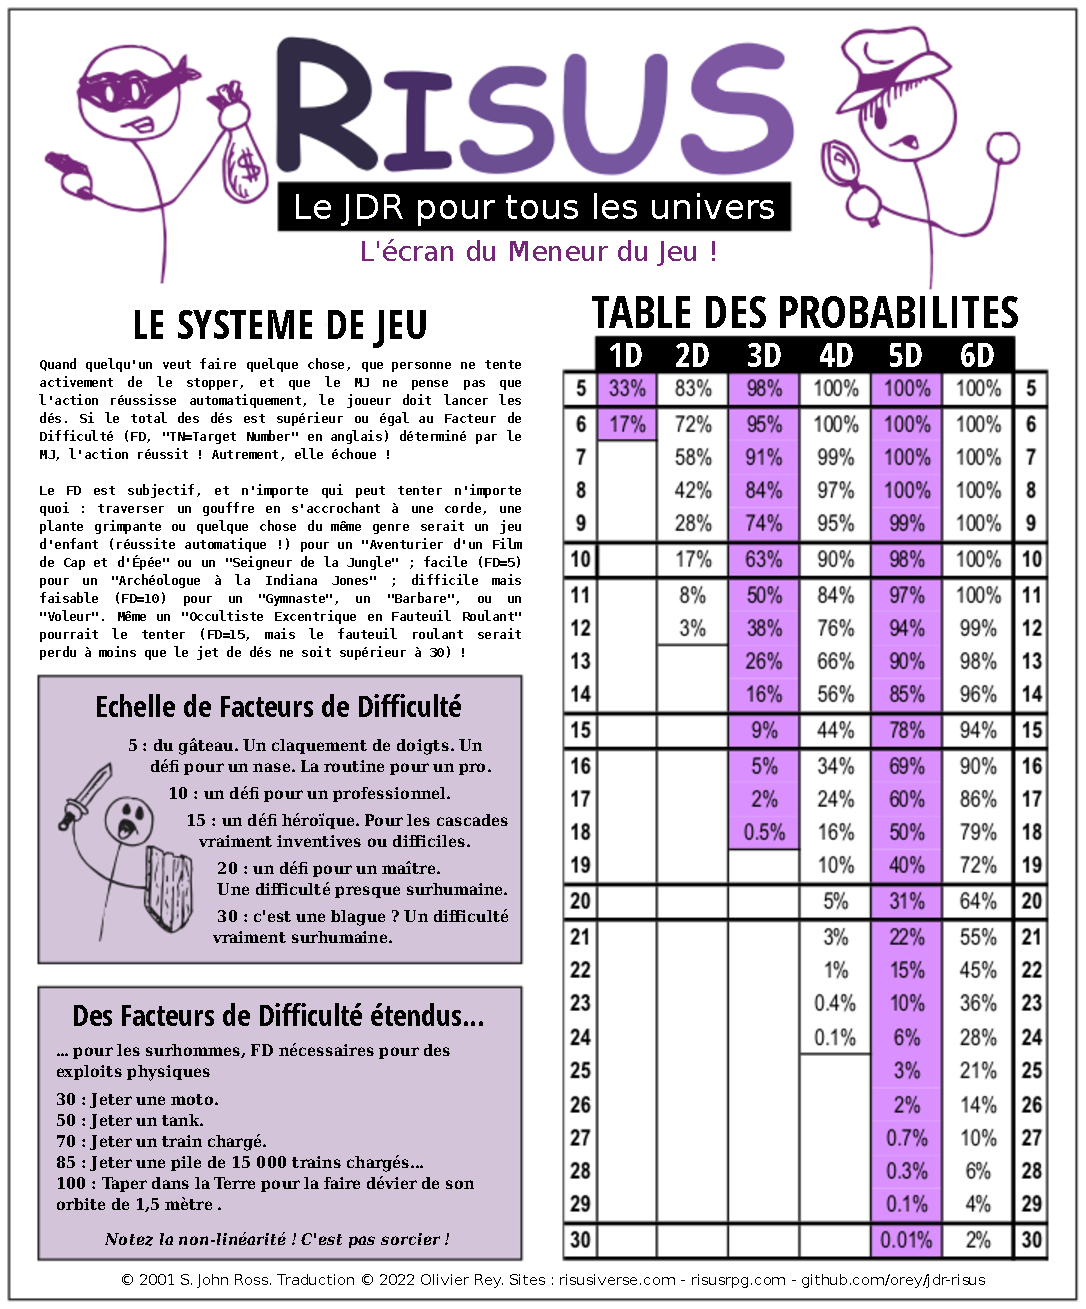
\includegraphics[page=1]{Risus-GM-Screen-fr-OReyJdr09.pdf}

\vfill

\begin{center}
\begin{tabular}{ll}
Risus en anglais  & \href{https://www.drivethrurpg.com/product/170294/Risus-The-Anything-RPG}{Risus the RPG} (c) Big Dice Games \\
Risus en français & \href{https://rouboudou.itch.io/risus}{Risus, traduction de Tristan Lhomme, plus aides de jeu} \\
Sites américains  & \href{https://www.risusrpg.com}{risusrpg.com} \\
                  & \href{https://www.risusiverse.com/}{risuiverse.com} \\
Copyleft    & \textcopyleft\ Olivier Rey 2022 \\
Référence   & \myreference\ -- Version \myversion \\
Publié sur  & \href{https://rouboudou.itch.io}{rouboudou.itch.io} \\
            & \href{https://github.com/orey/\myrepo}{github.com/orey/\myrepo} \\      
\end{tabular}
\end{center}

\end{frame}



\end{document}


